%! Author = ruochongli
%! Date = 2023/3/11

% Preamble
\documentclass[./main.tex]{subfiles}
% Packages

% Document
\begin{document}
    \section{Model Verification}
    To prove the mathematical model\rq{s} accuracy and effectiveness, we would verify it by selecting another location
    and put the
    raw information into the model.
    Then compare the model\rq{s} results with the actual choice of the decision makers.
    If the result is the same or similar, then the model should be accurate and effective.

    We choose a property in Malaysia to be the calibration.
    A satellite view of the property is provided in Figure~\ref{fig:figureClubMedWB} and Figure~\ref{fig:figureClubMedB}
    The property\lq{s} boundaries are defined by four roads and a beach:
    \begin{itemize}
        \item Northern boundaries: Jalan Bukit Cheraing
        \item Western boundaries: Laluan Presekutuan 3 \& Jalan Kampung Cherating Lama \& Jalan Pantai
        \item Southern boundaries: Cherating Beach
        \item Eastern boundaries: Cherating Beach
    \end{itemize}
    \begin{figure}[H]
        \centering
        \begin{minipage}{0.32\linewidth}
            \centering
            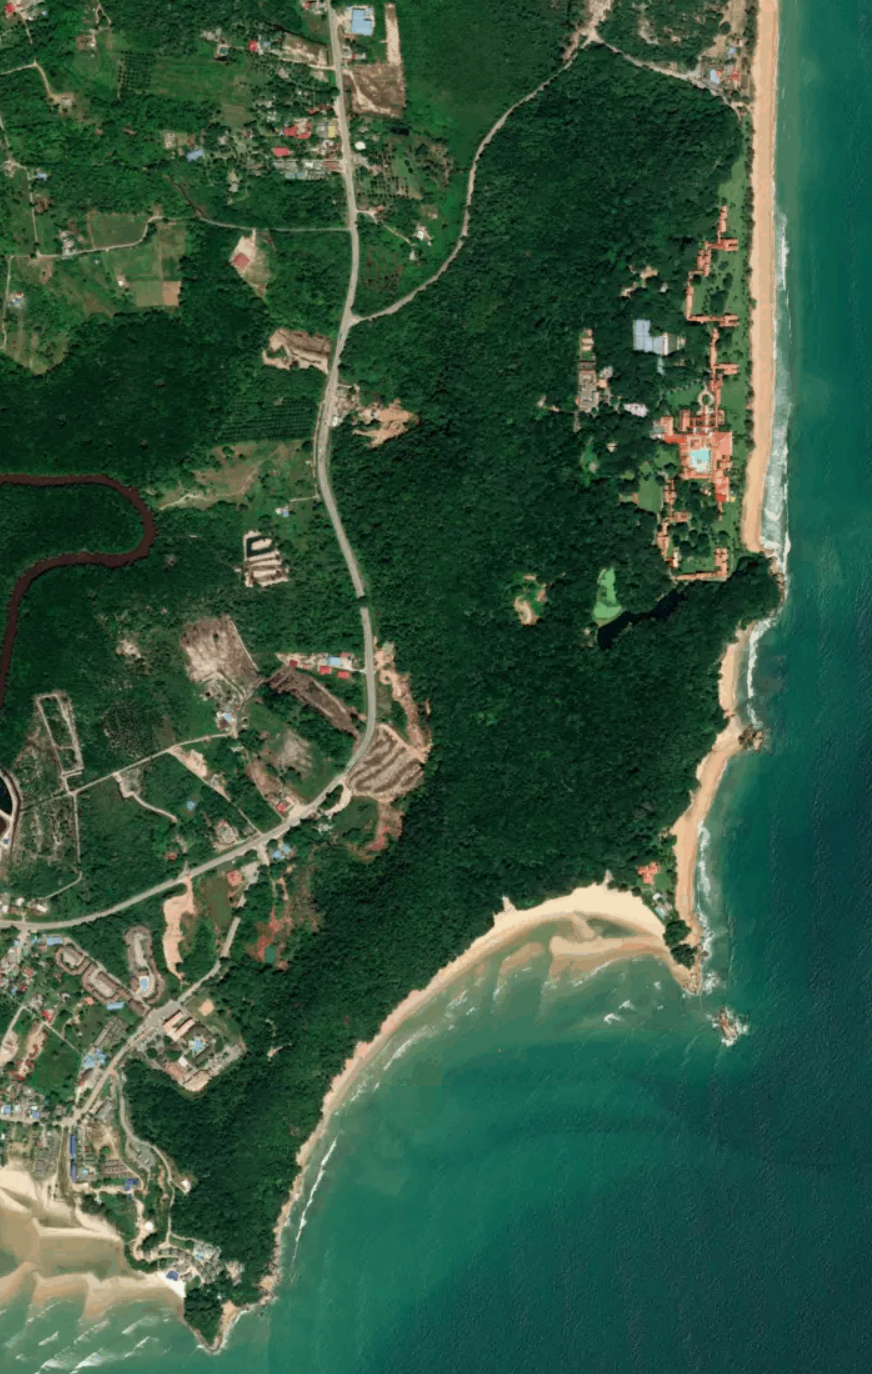
\includegraphics[width=0.75\linewidth]{./figure/figureClubMedMapWB}
            \caption{A satellite image of the parcel of land}
            \label{fig:figureClubMedWB}
        \end{minipage}
        \begin{minipage}{0.32\linewidth}
            \centering
            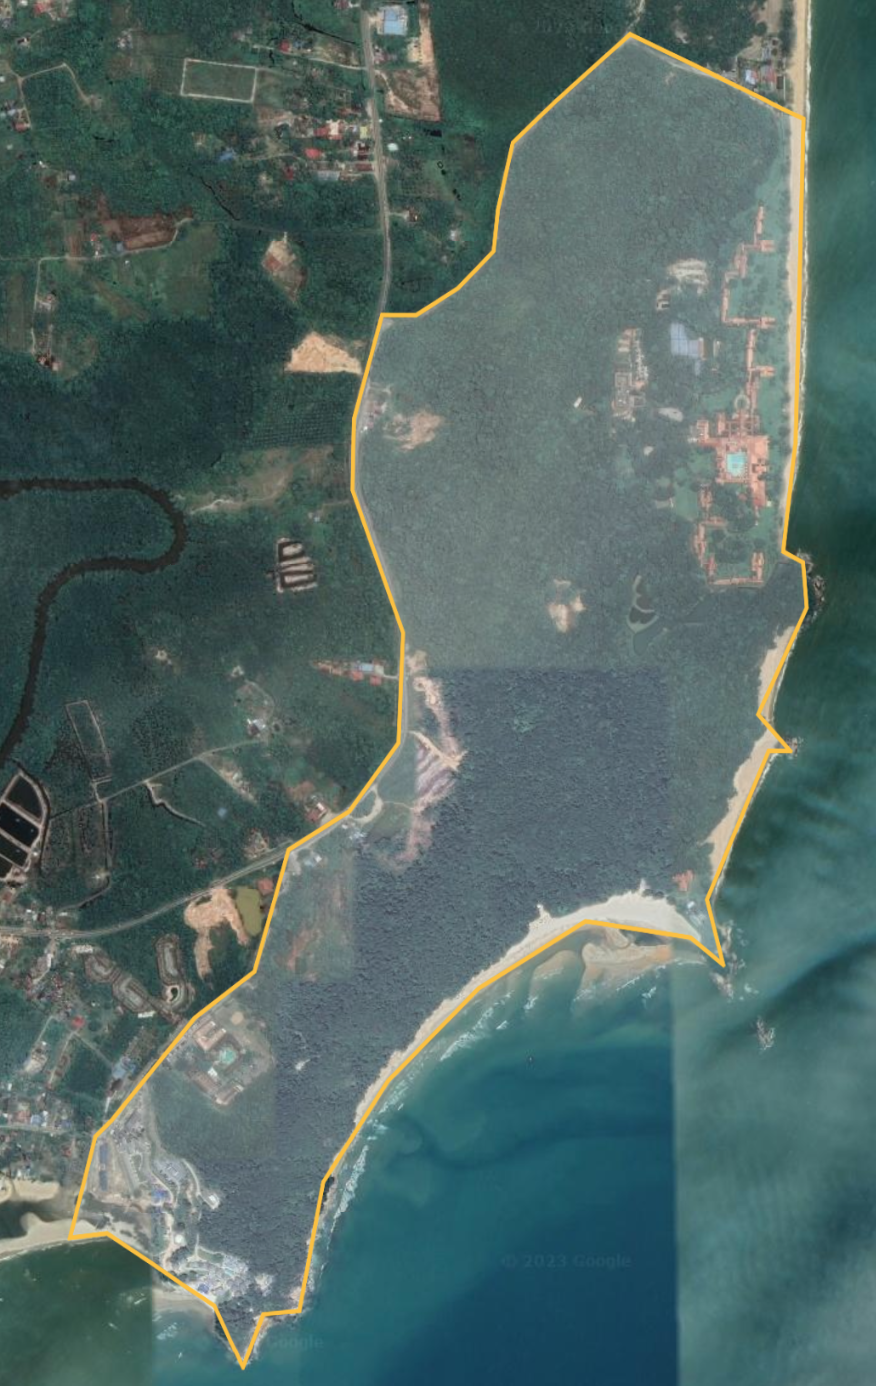
\includegraphics[width=0.75\linewidth]{./figure/figureClunMedB}
            \caption{Location of the parcel of land}
            \label{fig:figureClubMedB}
        \end{minipage}
        \begin{minipage}{0.32\linewidth}
            \centering
            \centering
            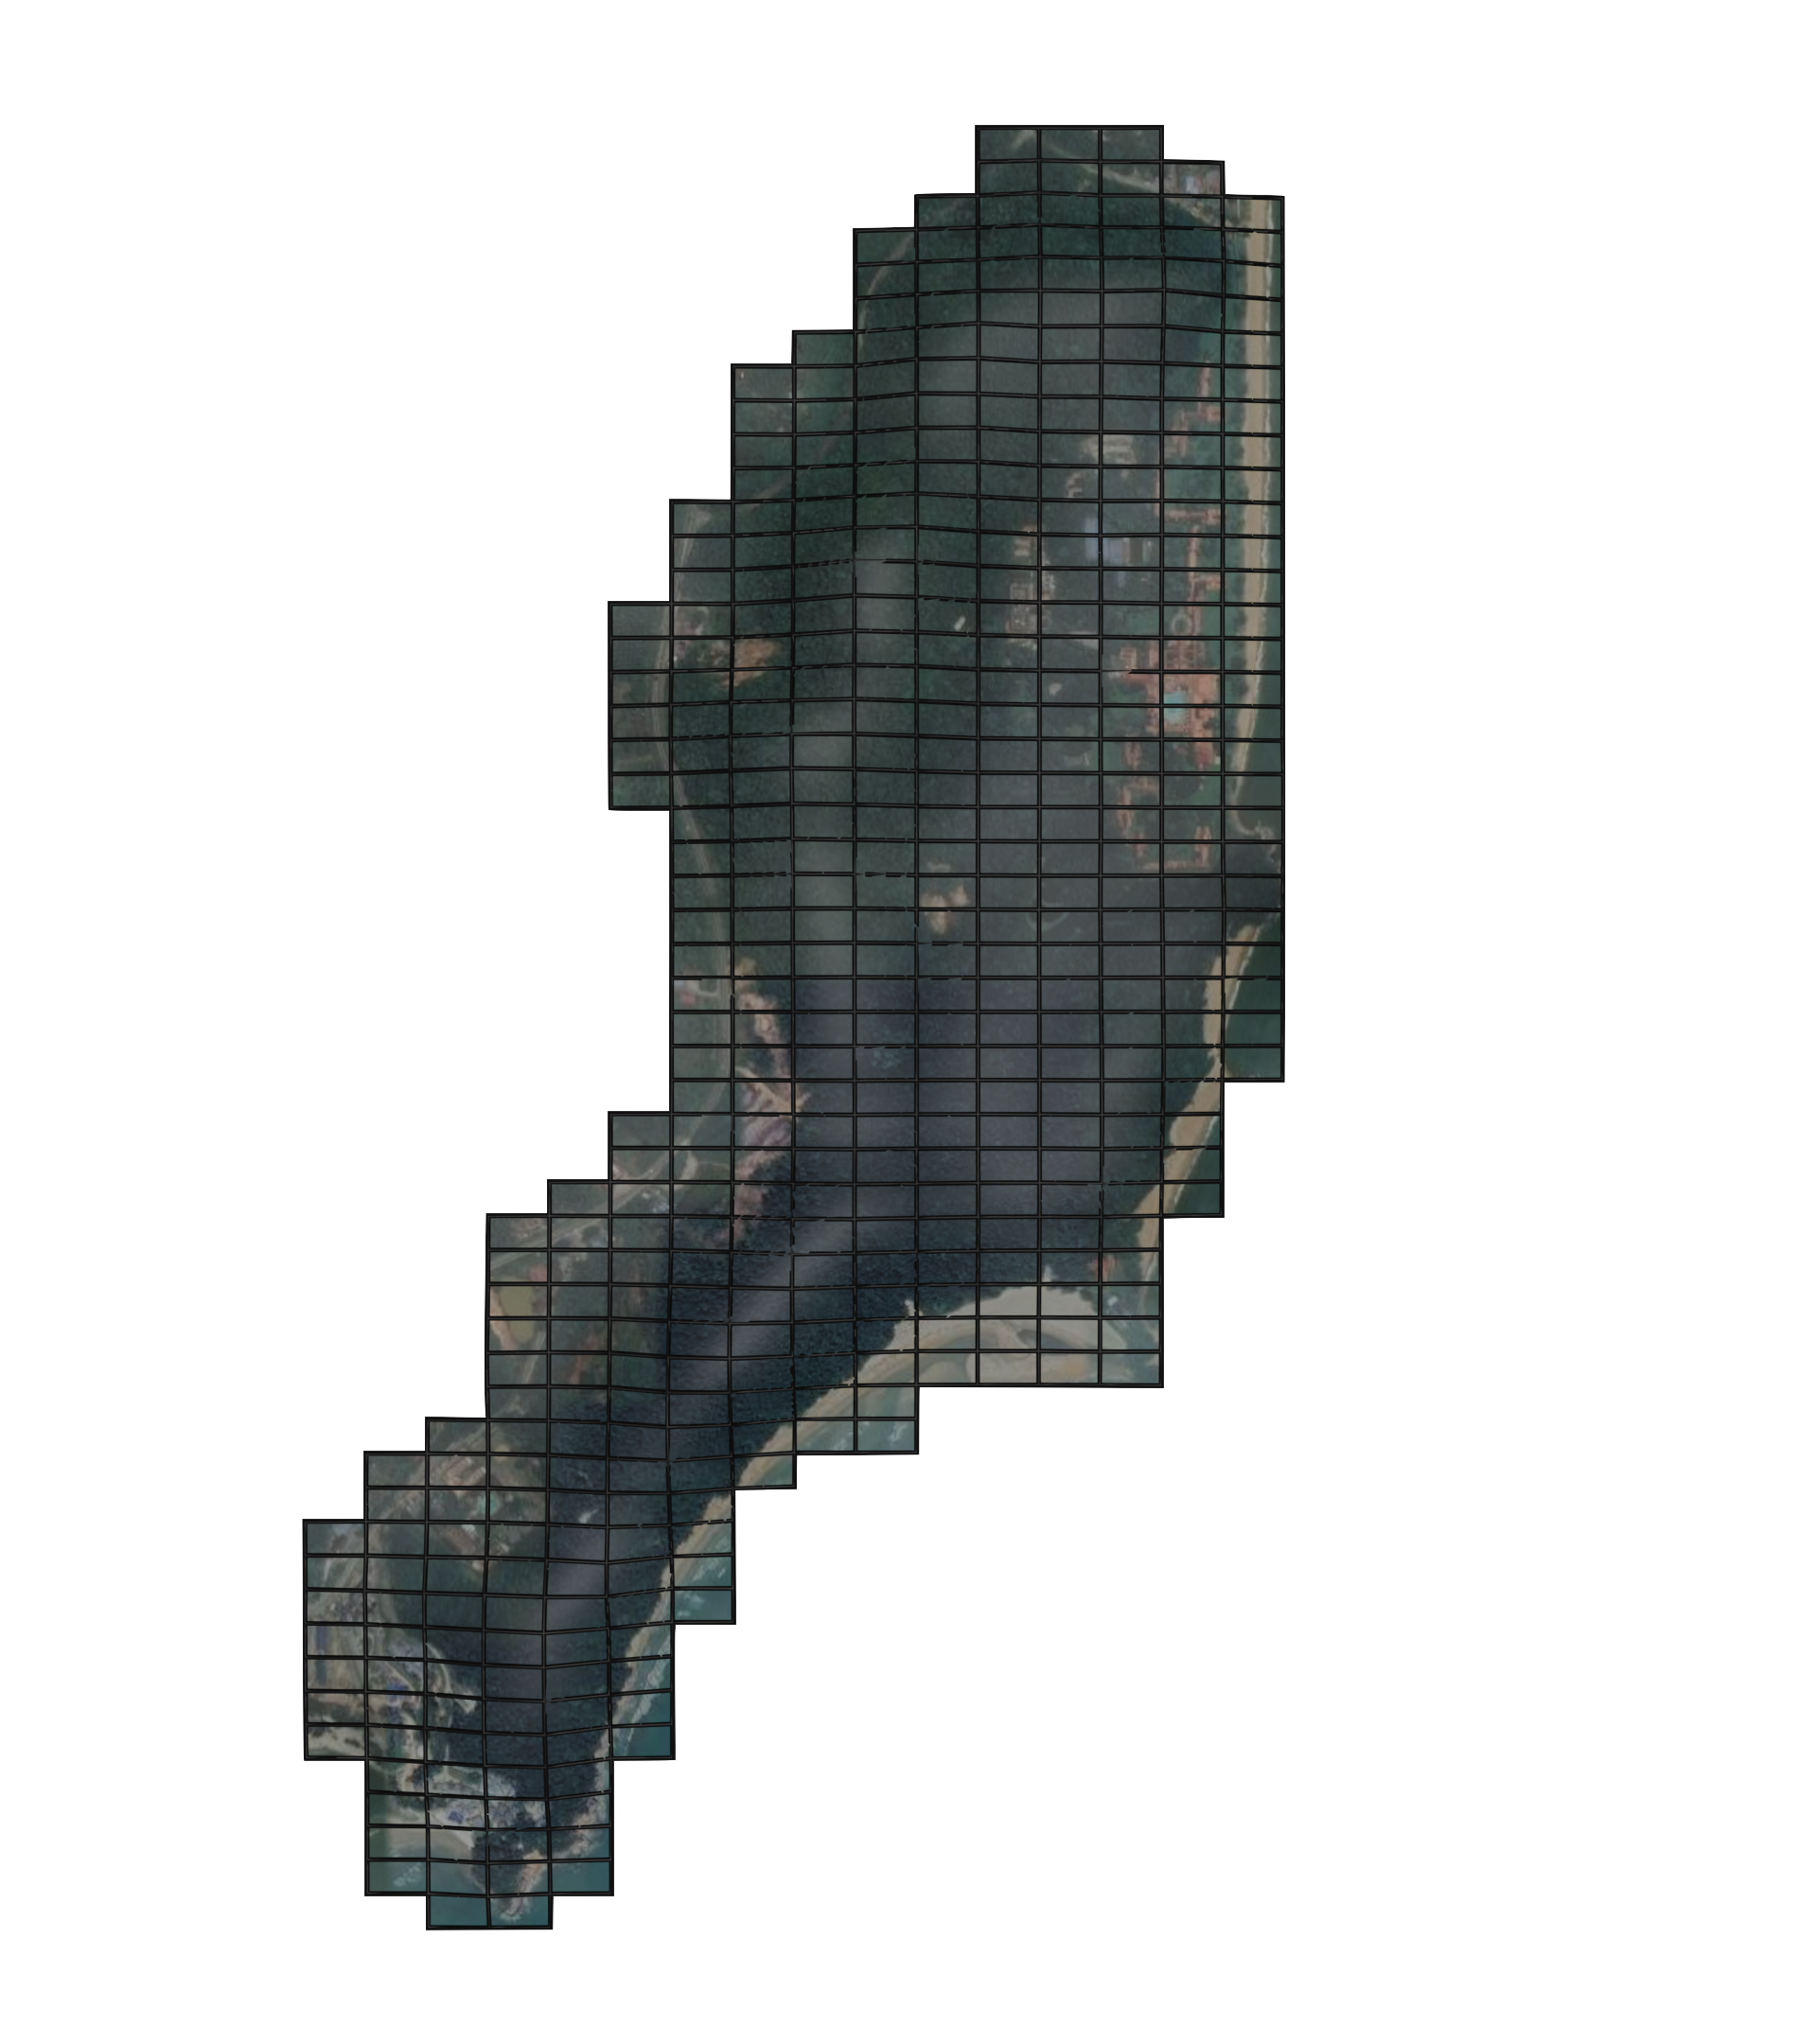
\includegraphics[width=1.05\linewidth]{./figure/figureClubMedStreight}
            \caption{A satellite image of the parcel of land}
            \label{fig:figureClubMedStreight}
        \end{minipage}
    \end{figure}

    \begin{figure}[H]
        \centering
        \includegraphics[width=0.75\linewidth]{./figure/figureClubMedAngle }
        \caption{Location of the parcel of land}
        \label{fig:figureClubMedAngle}
    \end{figure}

    This property can also be divided into $61$ meters by $35$ meters grids shown in
    Figure~\ref{fig:figureClubMedStreight} and Figure~\ref{fig:figureClubMedAngle}.
    The center of the property is located at $4\degree 8\rq$N $103\degree 24\rq$E in a rural tropical rainforest
    climate zone.
    The continental shelf is shallow, so it is not suitable for large ports for maritime transport.
    The river flows fast and the riverbed is meander, so it is also not suitable for either type of waterway
    transportation.
    Malaysia was lack of high-tech industries and scientific research capabilities, and cannot afford to build a
    research center; also, the area is humid and experiment equipments are prone to mold.
    Although Malaysia have Tin ores, this property is too close to the ocean thus very dangerous to mine
    , and
    likely to pollute the ocean.
    The surrounding area had a low population density in 1990 when the property was first planned.
    The forest is so dense to build expressways or railroads, thus inconvenient and inefficient to transport
    large amount of goods by land.
    For more information about this property, see Appendix A .

    In conclusion, it is not suitable for labor-oriented industries, raw-material-oriented
    industries, energy-oriented industries, power-oriented industries, and technology-oriented industries.
    The property is surrounded by hills and oceans on west and east side accordingly, so that it is
    not suitable for agriculture and animal husbandry.

    Taking the above into consideration, it is obvious that the property is neither suitable for agricultural nor
    industrial development.
    The option left is to develop service industries: including hotels.
    In reality, the property is currently dominated by Club Med Cherating Beach Hotel owned by the Fosun International.

    Our model suggests, when the property is covered with fields, the coefficient of profit $P$ is $37.9$ pts in
    Grade C;
    when covered with hotels, the coefficient of profit $P$ is $92.2$ pts in Grade A .

    Our model fits well with geographical analysis and the actual solution, and proved that out model is reasonably
    accurate and promotable.


\end{document}